\documentclass[11pt]{article}   % list options between brackets
\usepackage[utf8]{inputenc}
\usepackage[T1]{fontenc}
\usepackage{lmodern}
\usepackage[polish]{babel}
\usepackage{amsmath}
\usepackage{blindtext}
%\usepackage{amsfonts}
%\usepackage{amssymb}
\usepackage{subcaption}
\usepackage{float}
\usepackage{color}
\usepackage{wrapfig}
\usepackage{listings}
\usepackage{graphicx} % Allows including images
%\usepackage{booktabs} % Allows the use of \toprule, \midrule and \bottomrule in tables

% type user-defined commands here

\begin{document}
	\begin{titlepage}
	\title{%
		Projekt Rest Web Service\\
		\large Sklep internetowy z kartami do gry Magic: The Gathering\\
		Specyfikacja Wejście-Wyjście\\
	wersja 1.0}
	\author{Paweł Marczak i Łukasz Kosmaty}         % type author(s) between braces
	\date{\today}    % type date between braces
	\maketitle
	\end{titlepage}
	\tableofcontents
	\section{Wstęp}     % section 1.1
	%\subsection{History}       % subsection 1.1.1
	\subsection{Przeznaczenie}
	Celem zaprojektowanego web service-u jest automatyzacja procesu składania zamówień na karty w sklepie sprzedającym single (karty na sztuki) do gry Magic: The Gathering.\par W obecnej wersji, web service pozwala na przegląd magazynu sklepu (narazie zdefiniowanego statycznie),  uzupełnienie koszyka zamówienia przez użytkownika, złożenie zamówienia (z kontrolą poprawności zamówienia i odpowiednią aktualizacją stanu magazynu) oraz wydrukowanie potwierdzenia zamówienia w formacie pdf. By obslugiwać serwis można korzystać z przygotowanego przez nas klienta obsługiwanego za pośrednictwem html.\par Serwis został stworzony z myślą o dalszym rozwoju. Przykładowymi ścieżkami rozwoju są: integracja z zewnętrznymi bazami danych, możliwość otwartej rejetracji, szyfrowanie przesyłanych komunikatów (np. przy użyciu standardu SSL), integracja z zewnętrznymi systemami płatniczymi.
	\subsection{Zakres}
Dokument opisuje standardy sieciowe, według których zbudowana jest usługa oraz
prezentuje przykładowy sposób jej używania.
\section{Specyfikacja usługi Web Service}
Usługa ,,Sklep Mtg'' zaimplementowana została jako usługa sieciowa (Web
Service) z użyciem architektury Rest. \par
Usługa dostępna jest przez protokół HTTP (np. za pośrednictwem zaprojektowanego w HTML klienta).
	\subsection{Adres usługi}
	Usługa sklepu dostępna jest pod adresem \newline http://25.76.141.122:8080/RestProjectServer/webresources/sklep/ , a odpowiendnie metody do jego obsługi i ścieżki do nich zostaną opisane w dalszej części.
	\subsection{Specyfikacja wadl}
	 \lstset{
		language=xml,
		tabsize=3,
		%frame=lines,
		caption=Plik wadl,
		label=code:sample,
		frame=shadowbox,
		%rulesepcolor=\color{gray},
		xleftmargin=20pt,
		framexleftmargin=15pt,
		keywordstyle=\color{blue}\bf,
		commentstyle=\color{green},
		stringstyle=\color{red},
		numbers=left,
		numberstyle=\tiny,
		numbersep=5pt,
		breaklines=true,
		showstringspaces=false,
		basicstyle=\footnotesize,
		emph={food,name,price},emphstyle={\color{magenta}}}
\lstinputlisting{Plik_wadl.xml}
\subsection{Operacje usługi}
Usługa obsługuje operacje :
\begin{itemize}
	%\item zaloguj - zwraca informacje o koncie związanym z podanym loginem i hasłem
	\item getMagazyn - zwraca informacje o aktualnym stanie magazynu sklepu
	\item getStan- zwraca informacje o stanie pojedynczej pozycji z magazynu
	\item updateKoszyk - ustawia w koszyku klienta podaną liczbę kopii danej karty
	\item getKoszyk - zwraca informacje o aktualnym stanie koszyka klienta
	\item zwrocpozycjeZKoszyka-zwraca informacje o aktualnym stanie wybranej pozycji z koszyka klienta
	\item deleteFromKoszyk - usuwa z koszyka daną pozycję (wszystkie karty o danej nazwie)
	\item zlozZamowienie - składa zamówienie (weryfikuje poprawność koszyka, aktualizuje magazyn i stan konta użytkownika, wysyła informacje o potwierdzeniu zamówienia)
\end{itemize}
\subsection{Zwracane obiekty}
Szczegółowiej opisane zostaną tylko elementy budzące wątpliwości.
%\subsubsection{Konto}
%Obiekty zawierające informacje o zalogowanym użytkowniku, tzn.:
%\begin{itemize}
%	\item login (String)
%	\item haslo (String)
%	\item imie (String)
%	\item nazwisko (String)
%	\item stan\_konta (Float) - wirtualny stan konta służący do realizacji płatności
%	\item miasto (String)
%	\item kod\_pocztowy (String)
%	\item adres (String)
%	\item email (String)
%	\item numer\_telefonu (String)
%	\item ArrayList<Stan> koszyk- lista stanów w koszyku (karta+ liczba kopii karty+cena)
%	
%\end{itemize}
\subsubsection{Stan}
Obiekty zawierające informacje o danym stanie związanym z daną kartą(zarówno magazyn jak i koszyk klienta składają się z listy stanów ArrayList<Stan>), tzn.:
\begin{itemize}
	\item karta (Karta)- obiekt karta zawierający informacje o karcie
	\item na\_stanie (int) -liczba kopii karty karta w danym stanie
	\item cena (float)- cena pojedynczej kopii karty karta brutto
	\item wartosc\_razem- cena wszystkich kart w danym stanie brutto (cena*na\_stanie)
	
\end{itemize}
\subsubsection{Karta}
Obiekty zawierające informacje o danej karcie, tzn.:
\begin{itemize}
	\item nazwa (String)
	\item opis (String) - krótki opis karty: kolor, Set, rzadkość
	\item ilustracja (String)- grafika karty zakodowana w formacie Base64

	
\end{itemize}
\subsubsection{Magazyn}
Obiekty zawierające dane o stanie magazynu, tzn.:
\begin{itemize}
	\item ArrayList<Stan> lista\_st - lista stanów, z których złożony jest magazyn
\end{itemize}

\subsubsection{Potw\_zamowienia}
Obiekty zawierające informacje o statusie złożonego zamówienia, tzn.:
\begin{itemize}
	\item kwota (Float)- kwota brutto w pln.
	\item kwota\_netto(Float)- kwota netto w pln.
	\item dane\_klienta(Dane\_Klienta)- informacje o kliencie
	\item dane\_sklepu (Dane\_sklepu)- informacje o sprzedawcy.
	\item czy\_zatwierdzono(Boolean) -True, jeśli zamówienie zostało pomyślnie złożone, False- jeśli nie zostało pomyślnie złożone
	\item message (String)- komentarz dotyczący statusu zamówienia
\end{itemize}
\subsection {Implementacja HATEOAS (Hypermedia as the Engine of Application State)
}
Do zwracanych obiektów dodane zostały linki ułatwiające nawigowanie po usłudze. Są to dodatkowe elementy w formacie 
\begin{itemize}
	\item rel- String opisujący do czego odnosi się link
	\item uri- adres url do zasobu
\end{itemize}
\begin{figure}[H]
	\centering
	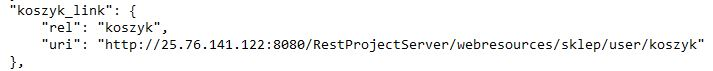
\includegraphics[width=0.8\linewidth]{komunikaty_zdjecia_rest/link}
	\caption{Przykładowy link zawarty w zwracanych obiektach}
	\label{zrzut0}
\end{figure}
\subsection{Specyfikacja wejście-wyjście opercji Web Service}
By operacje działały poprawnie użytkownicy muszą trzymać się określonych niżej standardów wyznaczonych przez nasz Restful Webservice.
%\subsubsection{Operacja zaloguj}
%Dane wejściowe:
%\begin{itemize}
%	\item login (String)- login skojarzony z kontem
%	\item haslo (String)- hasło skojarzone z kontem
%\end{itemize}	
%Dane wyjściowe:
%\begin{itemize}
%	\item obiekt typu Konto skojarzony z podanymi loginem i hasłem
%	\item zwraca wyjątek, jeżeli w bazie serwera nie ma konta o loginie i haśle podanych w zapytaniu
%\end{itemize}
\subsubsection{Nagłówki odpowiedzi}
Nagłówki każdej odpowiedzi serwisu składają się z 4 elementów, z których można odczytać m.in. format zawartości odpowiedzi. Postać nagłówka prezentuje się jak poniżej:
\begin{figure}[H]
	\centering
	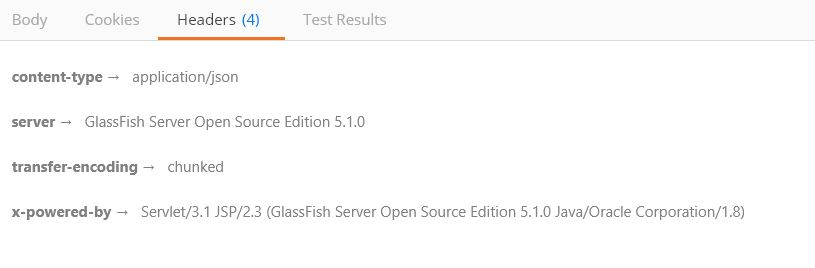
\includegraphics[width=0.8\linewidth]{komunikaty_zdjecia_rest/getMagazyn_res_head}
	\caption{Przykładowy nagłówek odpowiedzi serwisu}
	\label{zrzut1}
\end{figure}
\subsubsection{Operacja getMagazyn}
Dane wejściowe:
\begin{itemize}
	\item operacja GET
	\item ścieżka do operacji:http://25.76.141.122:8080/RestProjectServer/webresources/sklep
	\item pole login przekazane w nagłówku z loginem do obsługiwanego konta
	\item pole haslo przekazane w nagłówku z hasłem do obsługiwanego konta
\end{itemize}	
Dane wyjściowe:
\begin{itemize}
	\item obiekt typu Magazyn zgodny z aktualnym stanem magazynu sklepu
	\item zwraca wyjątek, jeżeli login i/lub hasło podane w nagłówku są nieprawidłowe

\end{itemize}


\begin{figure}[H]
	\centering
	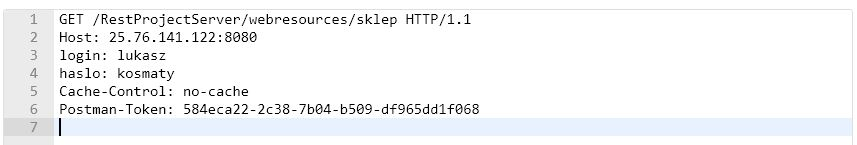
\includegraphics[width=0.8\linewidth]{komunikaty_zdjecia_rest/getMagazyn_req}
	\caption{Przykładowy HTTP request operacji zwrocMagazyn}
	\label{zrzut21}
\end{figure}
\begin{figure}[H]
	\centering
	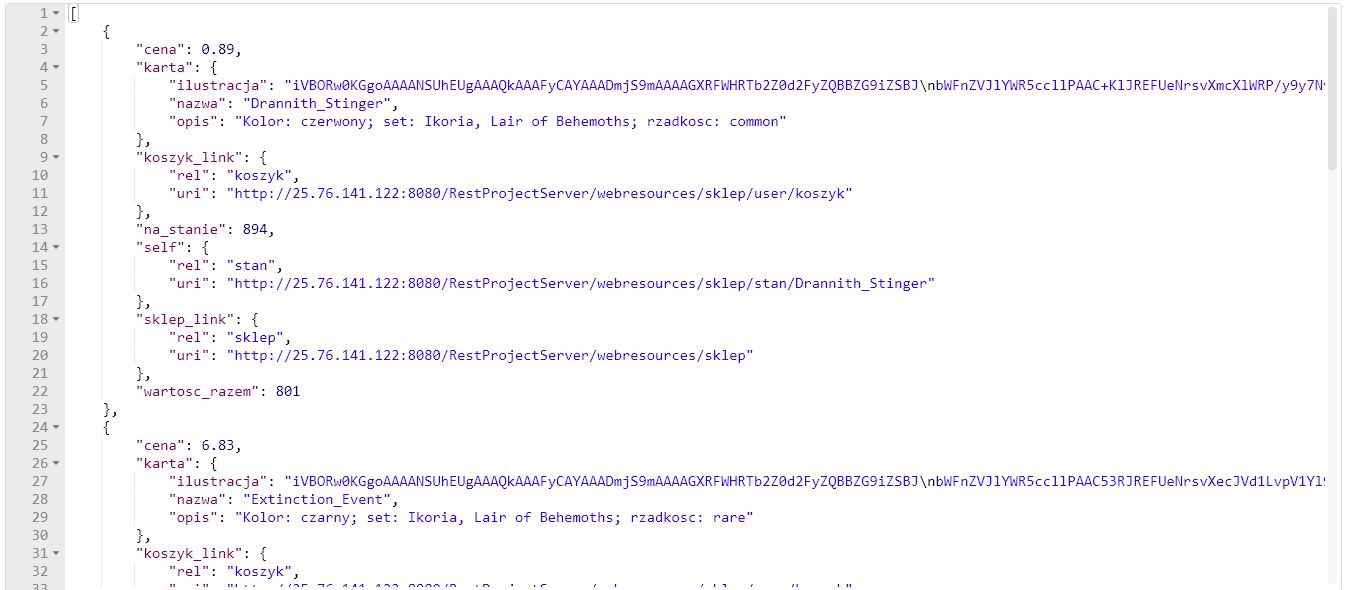
\includegraphics[width=0.8\linewidth]{komunikaty_zdjecia_rest/getMagazyn_res_body}
	\caption{Przykładowy response body (JSON) operacji zwrocMagazyn}
	\label{zrzut22}
\end{figure}
\subsubsection{Operacja getStan}
Zwraca wybraną pozycję z magazynu.
Dane wejściowe:
\begin{itemize}
	\item operacja GET
	\item ścieżka do operacji: \newline http://25.76.141.122:8080/RestProjectServer/webresources/sklep/\{nazwa karty\}
	\item nazwa karty (przekazana w ścieżce zapytania)
\end{itemize}	
Dane wyjściowe:
\begin{itemize}
	\item obiekt typu Stan zgodny z aktualnym stanem magazynu sklepu
	
\end{itemize}
\begin{figure}[H]
	\centering
	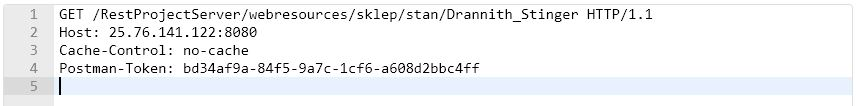
\includegraphics[width=0.8\linewidth]{komunikaty_zdjecia_rest/getStan_req}
	\caption{Przykładowy HTTP request operacji zwrocStan}
	\label{zrzut31}
\end{figure}
\begin{figure}[H]
	\centering
	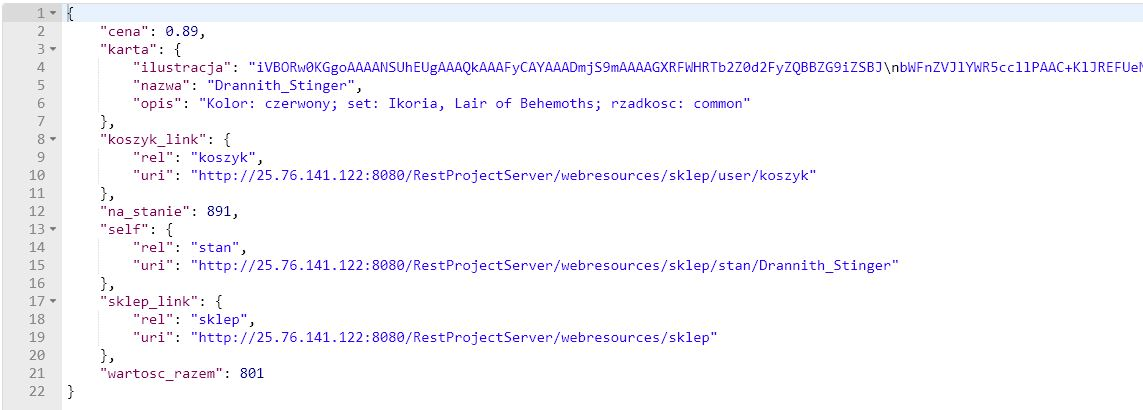
\includegraphics[width=0.8\linewidth]{komunikaty_zdjecia_rest/getStan_res_body}
	\caption{Przykładowy response body (JSON) operacji zwrocStan}
	\label{zrzut32}
\end{figure}

\subsubsection{Operacja updateKoszyk}
Operacja nie dodaje pozycji do koszyka, a ustawia w koszyku podaną przez klienta pozycję w podanej liczbie sztuk.\newline
Dane wejściowe:
\begin{itemize}
	\item operacja PUT
	\item ścieżka do operacji: \newline http://25.76.141.122:8080/RestProjectServer/webresources/sklep/\{nazwa karty\}?ilosc=\{liczba\}
	\item nazwa karty (przekazana w ścieżce zapytania)
\item liczba (int)- liczba kopii karty, którą chcemy ustawić w koszyku przekazana jako query param w ścieżce do odpowiedniej karty z magazynu
\end{itemize}	
Dane wyjściowe:
\begin{itemize}
	\item linki do sklepu i koszyka
	\item zwraca wyjątek, jeżeli nie ma karty o podanej nazwie w magazynie.
\end{itemize}
\begin{figure}[H]
	\centering
	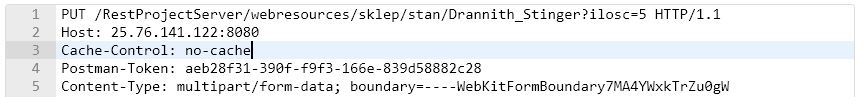
\includegraphics[width=0.8\linewidth]{komunikaty_zdjecia_rest/updateKoszyk_req}
	\caption{Przykładowy HTTP request operacji updateKoszyk}
	\label{zrzut41}
\end{figure}
\begin{figure}[H]
	\centering
	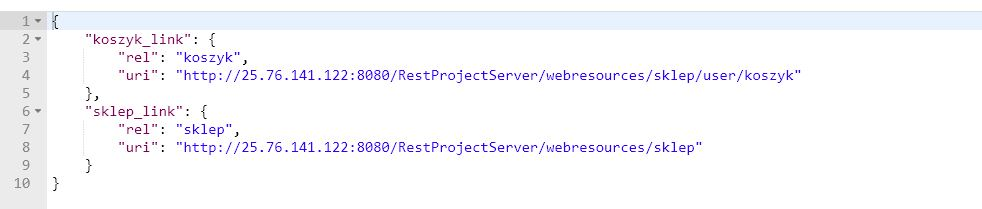
\includegraphics[width=0.8\linewidth]{komunikaty_zdjecia_rest/updateKoszyk_res_body}
	\caption{Przykładowy response body (JSON) operacji updateKoszyk}
	\label{zrzut42}
\end{figure}
\subsubsection{Operacja getKoszyk}
Dane wejściowe:
\begin{itemize}
	\item operacja GET
	\item ścieżka do \newline operacji:http://25.76.141.122:8080/RestProjectServer/webresources/sklep/user/koszyk
\end{itemize}	
Dane wyjściowe:
\begin{itemize}
	\item obiekt typu Koszyk zgodny z aktualnym stanem koszyka klienta

	
\end{itemize}


\begin{figure}[H]
	\centering
	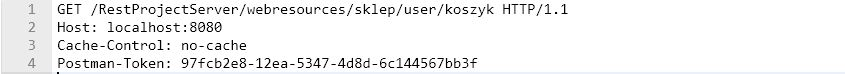
\includegraphics[width=0.8\linewidth]{komunikaty_zdjecia_rest/getKoszyk_req}
	\caption{Przykładowy HTTP request operacji getKoszyk}
	\label{zrzut51}
\end{figure}
\begin{figure}[H]
	\centering
	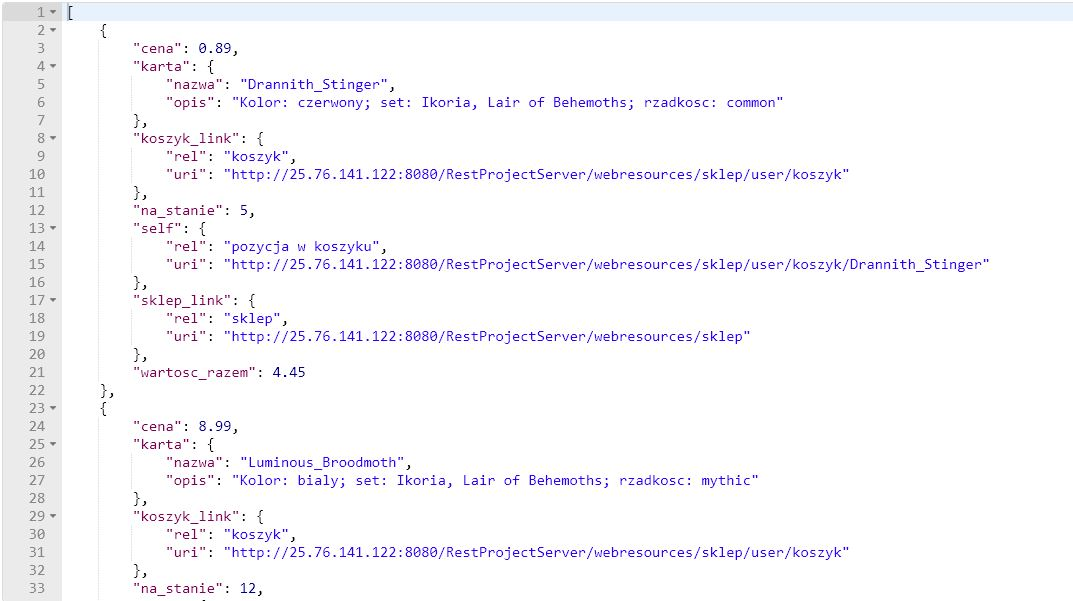
\includegraphics[width=0.8\linewidth]{komunikaty_zdjecia_rest/getKoszyk_res_body}
	\caption{Przykładowy response body (JSON) operacji getKoszyk}
	\label{zrzut52}
\end{figure}
\subsubsection{Operacja zwrocpozycjeZKoszyka}
Zwraca wybraną pozycję z koszyka. 
Dane wejściowe:
\begin{itemize}
	\item operacja GET
	\item ścieżka do operacji:\newline http://25.76.141.122:8080/RestProjectServer/webresources/sklep/user/koszyk\{nazwa karty\}
	\item nazwa karty (przekazana w ścieżce zapytania)
\end{itemize}	
Dane wyjściowe:
\begin{itemize}
	\item obiekt typu stan odpowiadający pozycji z koszyka
	
\end{itemize}
\begin{figure}[H]
	\centering
	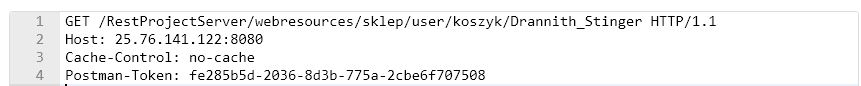
\includegraphics[width=0.8\linewidth]{komunikaty_zdjecia_rest/zwrocpozycjeZKoszyka_req}
	\caption{Przykładowy HTTP request operacji zwrocpozycjeZKoszyka}
	\label{zrzut61}
\end{figure}
\begin{figure}[H]
	\centering
	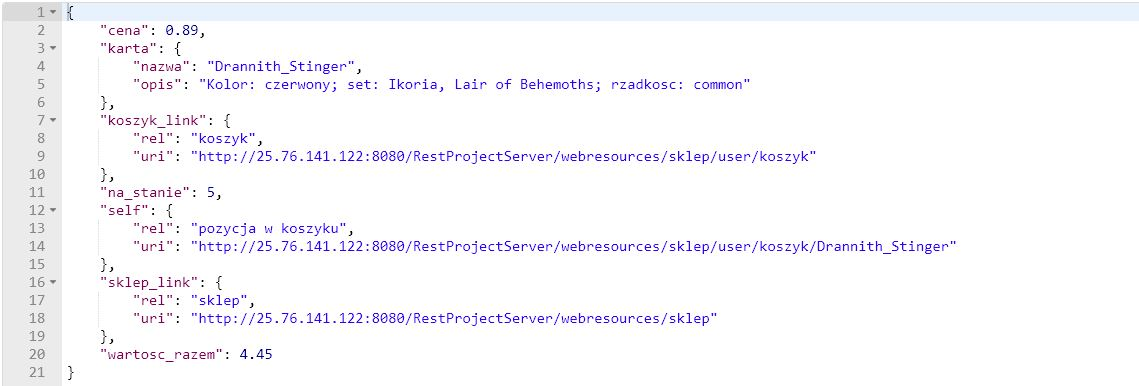
\includegraphics[width=0.8\linewidth]{komunikaty_zdjecia_rest/zwrocpozycjeZKoszyka_res_body}
	\caption{Przykładowy response body (JSON) operacji zwrocpozycjeZKoszyka}
	\label{zrzut62}
\end{figure}
\subsubsection{Operacja deleteFromKoszyk}
Operacja usuwa podaną pozycję z koszyka podanego konta.\newline
Dane wejściowe:
\begin{itemize}
	\item operacja DELETE
	\item ścieżka do operacji:\newline http://25.76.141.122:8080/RestProjectServer/webresources/sklep/user/koszyk/\{nazwa karty\}
	\item nazwa karty (przekazana w ścieżce zapytania)

\end{itemize}	
Dane wyjściowe:
\begin{itemize}
	\item zwraca linki do sklepu i koszyka
	\item zwraca wyjątek, jeżeli w bazie serwera nie ma konta o loginie i haśle podanych w zapytaniu, lub nie ma karty o podanej nazwie w koszyku.
\end{itemize}
\begin{figure}[H]
	\centering
	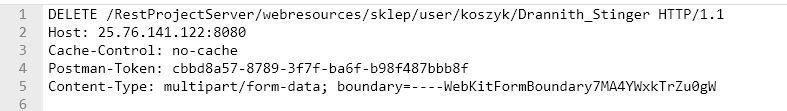
\includegraphics[width=0.8\linewidth]{komunikaty_zdjecia_rest/deleteFromKoszyk_req}
	\caption{Przykładowy HTTP request operacji deleteFromKoszyk}
	\label{zrzut71}
\end{figure}
\begin{figure}[H]
	\centering
	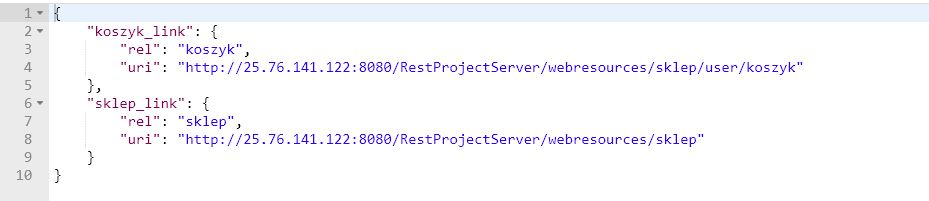
\includegraphics[width=0.8\linewidth]{komunikaty_zdjecia_rest/deleteFromKoszyk_res_body}
	\caption{Przykładowy response body (JSON) operacji deleteFromKoszyk}
	\label{zrzut72}
\end{figure}

\subsubsection{Operacja zlozZamowienie}
Operacja sprawdza poprawność koszyka (spójność z magazynem), stan konta użytkownika i zwraca potwierdzenie transakcji oraz aktualizuje stan magazynu i opróżnia koszyk.\newline
Dane wejściowe:
\begin{itemize}
	\item operacja POST
	\item ścieżka do operacji:\newline http://25.76.141.122:8080/RestProjectServer/webresources/sklep/user/koszyk
	
\end{itemize}	
Dane wyjściowe:
\begin{itemize}
	\item obiekt typu Potw\_zamowienia z wszelkimi informacjami dotyczącymi transakcji
	\item jeżeli zamówienie nie zostało potwierdzone, wtedy w potwierdzeniu zwracane jest czy\_zatwierdzono = False i komentarz w polu message.
\end{itemize}
\begin{figure}[H]
	\centering
	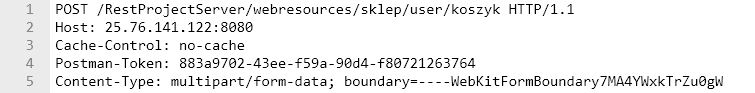
\includegraphics[width=0.8\linewidth]{komunikaty_zdjecia_rest/zlozZamowienie_req}
	\caption{Przykładowy HTTP request operacji zlozZamowienie}
	\label{zrzut81}
\end{figure}
\begin{figure}[H]
	\centering
	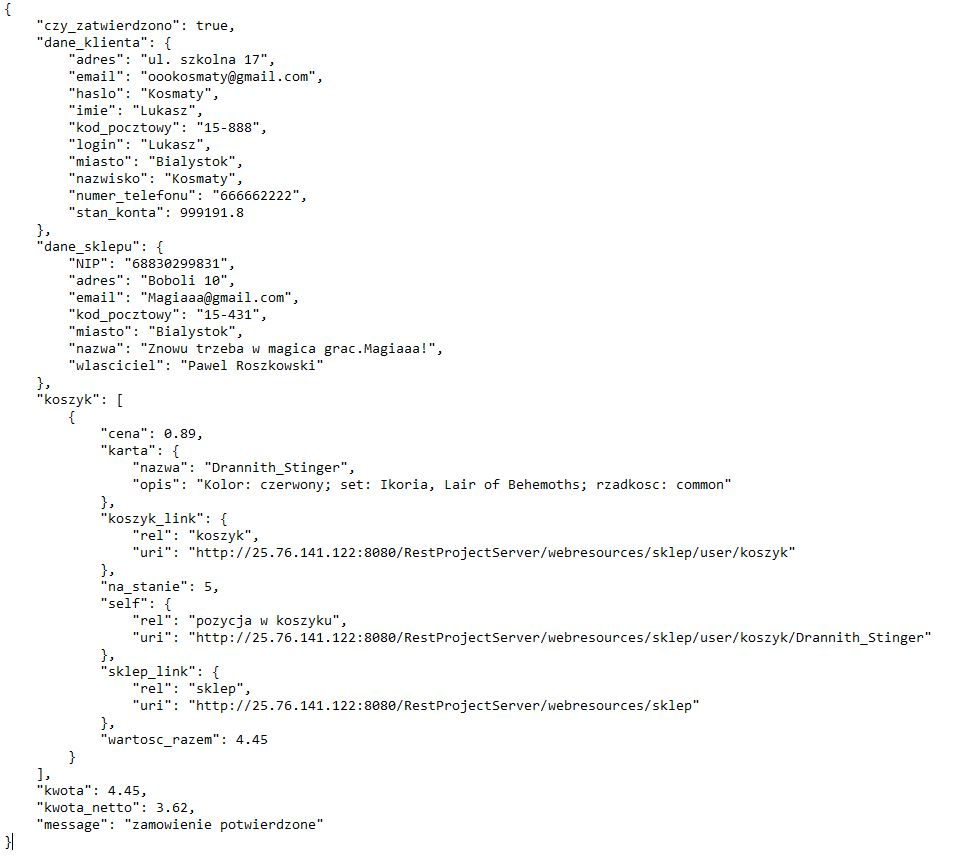
\includegraphics[width=0.8\linewidth]{komunikaty_zdjecia_rest/zlozZamowienie_res_body}
	\caption{Przykładowy response body (JSON) operacji zlozZamowienie}
	\label{zrzut82}
\end{figure}

\end{document}
